\section{Gesamtsystem}\label{gesamtsystem}
Die komplette Datenpipeline von dem Server des DWD bis zur Darstellung in der App sieht wie folgt aus.  

\begin{figure}[htb]
 \centering
 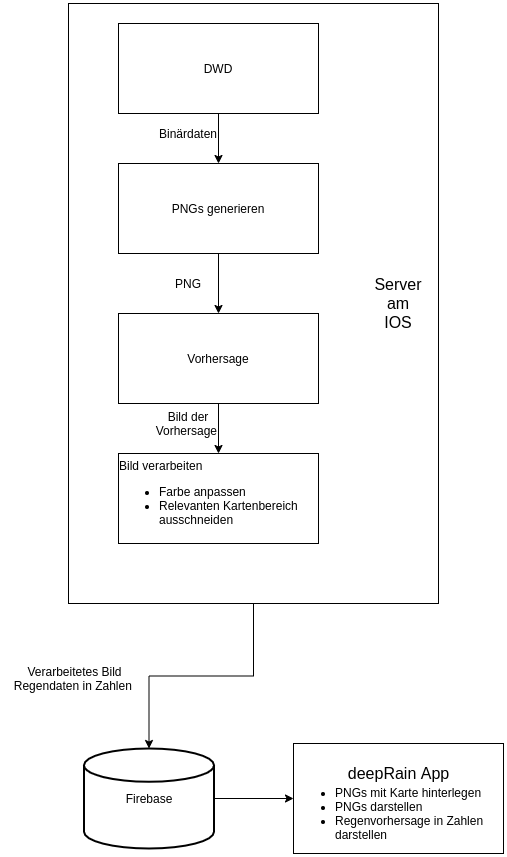
\includegraphics[width=0.6\textwidth,angle=0]{abb/Gesamtsystem}
 \caption[Das Gesamtsystem]{Das Gesamtsystem}
\label{fig:Beschreibung}
\end{figure}

Der DWD stellt alle fünf Minuten die neusten Regendaten für Deutschland im Binär Format zur Verfügung. Diese werden heruntergeladen und in der Datenaufbereitung verwendet um PNGs zu generieren (Siehe Kapitel “Datenaufbereitung”). Dieses PNGs werden im Anschluss verwendet um eine Regenvorhersage zu machen (Siehe Kapitel “Regenvorhersage / Netze”). Der Output der Regenvorhersage ist wieder ein PNG. Dieses PNG wird in der Firebase gespeichert und auf allen Geräten mit der installierten App angezeigt. Außerdem wird für alle Regionen in der die App verwendet wird eine Regenvorhersage in Zahlenform hochgeladen und auf den jeweiligen Geräten angezeigt (Siehe Kapitel “App und Datenbank”). 
Der Übersichtlichkeit halber haben wir das gesamte Projekt in die drei Komponenten “Datenbeschaffung |\& Vorverarbeitung”, “Vorhersage” und “App |\& Datenbankhandling” aufgeteilt.  
Die Komponente “Datenbeschaffung |\& Vorverarbeitung” beinhaltet alles vom Download der Daten beim DWD bis zu den daraus generierten PNG’s. In der Komponente “Vorhersage” werden die Regenvorhersage mithilfe von neuronalen Netzen gemacht. In der Komponente “App |\& Datenbankhandling” geht es um das Datenmanagement mit Firebase, wie die Daten dort hingelangen und um die App welche die Daten darstellt.  
(Hier sollten wir gegen Ende des Projektes eventuell noch ein bisschen genauer beschreiben wie das alles genau funktioniert. Das wird unseren Nachfolgern sehr stark helfen um sich schnell einzuarbeiten)  